\chapter{Tools Review}
\label{chapter:tools_review}

This chapter covers a review of the experimental setup and relevant software tools helpful in developing the final solution.

\section{Experimental Setup}

The experimental part of this thesis was developed using the setup available at the Laboratory for Automation and Robotics (LAR) located in the Department of Mechanical Engineering at the University of Aveiro. The available setup contains an UR10e collaborative robot with an Orbbec Astra Pro RGBD camera above the workspace.

\textcolor{red}{Robot and Camera images here}

All communication is set up using ROS with Rviz being used to help visualize the functioning of the system. Additionally, the MoveIt! framework was used to take care of the planning of the robot movements.

\section{\acf{ros}}

\acs{ros}\cite{ROS2}\footnote{\acs{ros} 1 documentation: \url{https://wiki.ros.org}}\footnote{\acs{ros} 2 documentation: \url{https://docs.ros.org/en/humble}} is an open-source collection of tools and software libraries used to develop a robotics application. Its main features are:

\begin{itemize}
    \item \textbf{message broker}: every process in the project is a node in the \acs{ros} network and communicates with the other nodes mainly through topics (asynchronous publish/subscribe streaming of data) or services (synchronous RPC-style communication);
    \item \textbf{code reuse}: executables and packages are written to be as independent as possible, making the developer able to reuse them in another project;
    \item \textbf{rich ecosystem}: there are several open-source packages available to the developer that can be easily integrated;
    \item \textbf{scalability}: given that the nodes are so loosely coupled, it allows for node distribution;
    \item \textbf{language independence}: nodes can be written in any language since communication is established through well-defined objects;
    \item \textbf{data visualization}: there are tools to visualize the data in real-time, such as Rviz;
    \item \textbf{simulator support}: \acs{ros} has support for simulators with Gazebo being the most common;
    \item \textbf{hardware abstraction}: contains driver packages to deal with some hardware devices;
\end{itemize}

\acs{ros} can be used by installing on Ubuntu or Mac OS X systems, and then nodes can be launched from existing repositories or can be programmed in Python, C++ or Lisp with more languages still under development.

\section{Machine Learning Frameworks}

This section contains a review of Tensorflow and Pytorch, which are two of the most popular machine learning frameworks that can be helpful in pre-processing data, building machine learning models and deploying said models.

\subsubsection{Tensorflow}

Tensorflow\footnote{Tensorflow documentation: \url{https://www.tensorflow.org/api_docs}} is a platform that can be used for all steps of a machine learning project. Its main features are:
\begin{itemize}
    \item \textbf{prepare data}: load data, data pre-processing and data augmentation;
    \item \textbf{build models}: design and train custom models with little code or use pre-trained ones (transfer learning);
    \item \textbf{deploy models}: helps using models in different platforms such as locally, in the cloud, in a browser, or in mobile;
    \item \textbf{implement MLOps}: run models in production, tracking their performance and identifying issues.
\end{itemize}

Tensorflow can be used through its APIs in several languages to adapt to every project but the Python API is recommended since it is the most stable.

\subsubsection{Pytorch}

Pytorch\footnote{Pytorch documentation: \url{https://pytorch.org/docs}} is an open-source framework that can be used for all steps of a machine learning project. Its main features are:

\begin{itemize}
    \item \textbf{distributed model training}: takes advantage of some Python and C++ features to optimize the performance in both research and production phases;
    \item \textbf{robust ecosystem}: there are tools and libraries that extend PyTorch to include features related to, for example, computer vision and natural language processing;
    \item \textbf{ready for production}: it has tools to deploy models with scalability in environments such as the cloud;
    \item \textbf{cloud support}: it has good support in the most common cloud platforms allowing an easier deployment in a production environment.
\end{itemize}

Pytorch can be used through its APIs in Python, Java, or C++.

\section{Key Point Detection Frameworks}
\label{section:keypointdetection}

This section reviews OpenPose and OpenPifPaf which are two projects containing models to detect key points in images, such as the human skeleton joints.

\subsubsection{OpenPose}

OpenPose\cite{Cao2021,Simon2017,Cao2018,Wei2016}\footnote{OpenPose documentation: \url{https://cmu-perceptual-computing-lab.github.io/openpose}} is an open-source project that aims to detect key points in the human body, face, hands, and feet from images. Its main features are:

\begin{itemize}
    \item 2D real-time key point detection based on the body/foot, the hand, or the face of multiple people;
    \item 3D real-time key point detection based on images from multiple cameras of one person;
    \item estimation of camera calibration parameters;
    \item single-person tracking.
\end{itemize}

OpenPose can be used through the command-line or using an API for Python or C++.

\begin{figure}[h]
\centerline{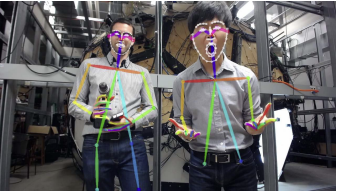
\includegraphics[height=1.55in]{figs/openpose.jpeg}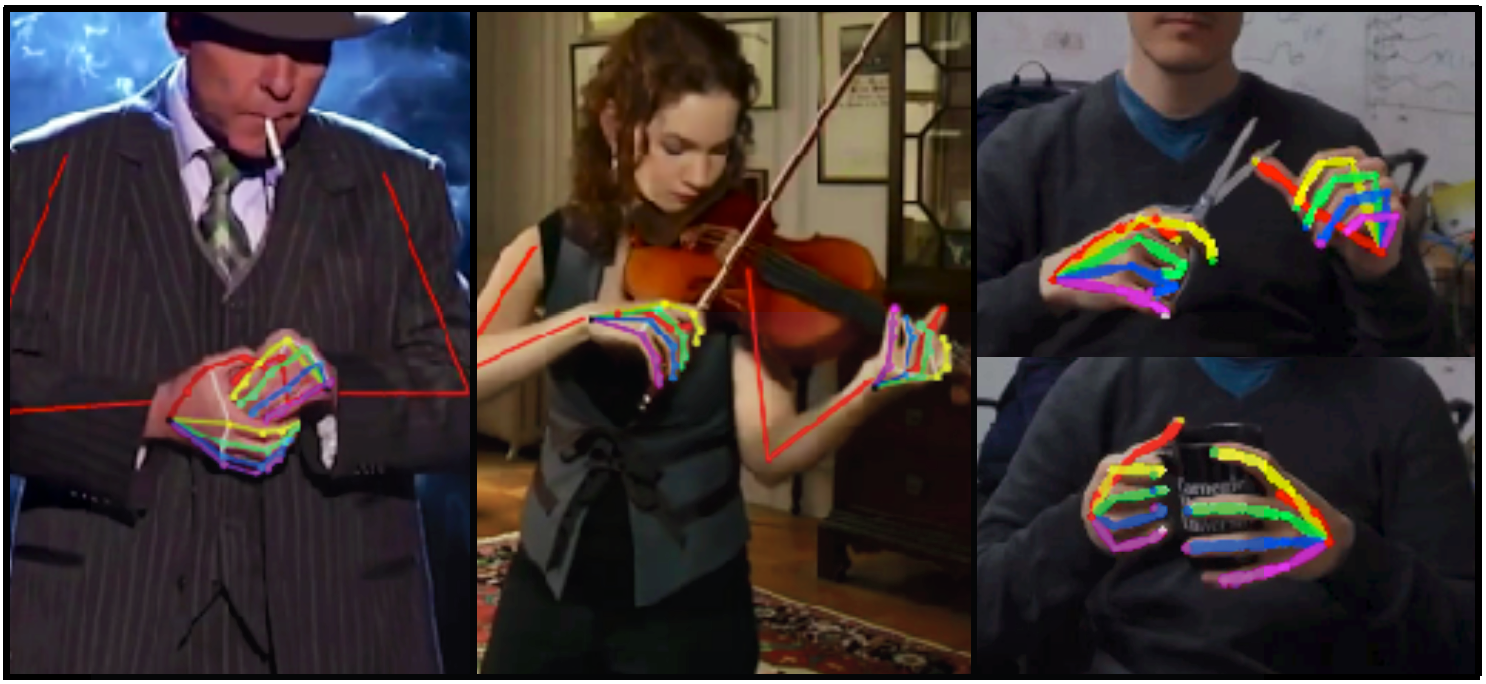
\includegraphics[height=1.55in]{figs/openpose2.PNG}}
\caption[OpenPose Examples]{OpenPose Examples \cite{Cao2021,Simon2017}}
\label{openpose}
\end{figure}

\subsubsection{OpenPifPaf}

OpenPifPaf\cite{Kreiss2021,Kreiss2019}\footnote{OpenPifPaf documentation: \url{https://openpifpaf.github.io}} is an open-source project that aims to detect, associate and track semantic key points. Detecting human joints is an example of its usage but it is also able to generalize this detection to other classes such as cars and animals. It can be installed as a python package which can then be imported.

\begin{figure}[h]
\centerline{\includegraphics[height=1.8in]{figs/openpifpaf.jpeg}}
\caption[OpenPifPaf Example]{OpenPifPaf Example \cite{Kreiss2021}}
\label{openpifpaf}
\end{figure}